\chapter{First-Order Reversal Curve (FORC) Diagrams of Nanomagnets with Cubic Magnetocrystalline Anisotropy}
\label{ch:res-2}
\fancyhead[L]{Single-domain FORC diagrams}
\fancyhead[C]{}
\fancyhead[R]{}
\fancyfoot[C]{\thepage}

\section*{Abstract}
First-order reversal curve (FORC) diagrams are increasingly used as a material's magnetic domain state fingerprint. FORC diagrams of noninteracting dispersions of single-domain (SD) particles with uniaxial magnetocrystalline anisotropy (MCA) are well studied. However, a large class of materials possess a cubic MCA, for which the FORC diagram properties of noninteracting SD particle dispersions are less understood. A coherent rotation model was implemented to study the FORC diagram properties of noninteracting ensembles of SD greigite (Fe$_3$S$_4$), and iron (Fe). FORC diagrams contain mixed information of irreversible and reversible rotations of the magnetisations. The pattern formation mechanism is identified and related to the irreversible events the individual particles undergo. The purely reversible signal is determined based on the FORC diagram properties of the individual particles. Our results support the utility of FORC diagrams for the identification of noninteracting to weakly-interacting SD particles with cubic MCA.\par

%%%%%%%%%%%%%%%%%%%%%%%%%%%%%%%%%%%%%%%%%%%%%%%%%%%%%%%%%%%%

\section{Introduction}
Ferromagnetic materials exhibit magnetic hysteresis: the dependence of the material's magnetisation $\boldsymbol{M}$ on its magnetic history \citep{Mayergoyz1986}. The hysteretic response of a material is obtained by a series of measurements of its scalar magnetisation $M=\boldsymbol{M} \cdot \boldsymbol{\hat{n}}$ as a function of the applied magnetic field $\boldsymbol{H}=H\boldsymbol{\hat{n}}$. To trace a hysteresis loop the magnetic field strength $H$ is slowly decreased from its saturation value $H=H_{\text{sat}}$ down to $H=-H_{\text{sat}}$, followed by the slow increase up to $H=H_{\text{sat}}$.\par

First-order reversal curves (FORCs) are a set of partial hysteresis loops, each starting at a saturation field $H=H_{\text{sat}}$, followed by the quasi-static decrease of the applied field strength down to $H=H_a$. From $H_a$, the field strength is increased back to $H=H_{\text{sat}}$ to trace a given curve labelled by its $H_a$ value. On each FORC, the scalar magnetisation is then a function $M=M(H_b, H_a)$ of the applied field $H=H_b$ and the $H_a$ value of the given curve ($H_a \leq H_b$).\par
The FORC distribution, an empirical analog of the Preisach weight function based on the experimental protocol described above, is defined as the second order mixed partial derivative \citep{Roberts2000}
\begin{equation}\label{forc}
\rho = \rho(H_b, H_a) = -\frac{1}{2}\frac{\partial^2 M}{\partial H_a \partial H_b},
\end{equation}
which must be understood in some weak sense to allow the discontinuous $M$. Contour plots of the FORC distribution (Eqn. \ref{forc}) are known as FORC diagrams and have been increasingly used by the wide magnetics community as a proxy for the magnetic domain state and switching behaviour of a variety of magnetic systems \citep{Pike1999,Pike2005,Roberts2000,Biasi2016,Proenca2017}.\par

Based on Stoner-Wohlfarth theory \citep{Stoner1948} significant progress has been made towards understanding the contribution of fine magnetic single-domain (SD) particles with uniaxial magnetocrystalline anisotropy (MCA) to the FORC diagram properties of interacting and noninteracting dispersions \citep{Newell2005,Egli2010,Biasi2016}. However, many materials including the most abundant ferromagnetic minerals on Earth possess a cubic MCA.\par

The general hysteretic properties of noninteracting dispersions of particles with cubic MCA has been previously studied \citep{Usov1997,Walker1993}. The cubic MCA system is more complicated than the uniaxial due to the existence of more local energy minima (LEM) and the mechanism behind the FORC diagram pattern formation is not yet as well understood as the uniaxial case.\par

Previous studies of FORC diagram pattern formation by minerals with cubic MCA used micromagnetics \citep{Muxworthy2004} and dipole-dipole modelling \citep{Harrison2014} to study the influence of magnetostatic interactions on the FORC diagram. However, the fully noninteracting case remains unknown as these studies rely on specific arrangements of particles positions and orientations, thus by definition cannot completely isolate the purely noninteracting contribution.\par

In this study we present an approach for numerically calculating the FORC diagram of a uniform noninteracting dispersion of SD particles with cubic MCA. The magnetic parameters of: greigite (Fe$_3$S$_4$), saturation magnetisation $M_s=2.7\times 10^5 \, \text{A/m}$ \citep{Li2014} and first anisotropy constant $K_1=-1.7\times 10^4 \, \text{J/m}^3$ \citep{Winklhofer2014}; and metallic iron (Fe), $M_s=1.7\times 10^6 \, \text{A/m}$ \citep{Dunlop} and $K_1=4.8\times 10^4 \, \text{J/m}^3$ \citep{Graham1958} have been used due to their opposing $K_1$ signs, their relatively high anisotropy and their importance for technological applications as well as the Earth sciences.\par

\section{Method}
\subsection{The FORC model}
In an ensemble of identical, randomly aligned particles the probability of a given particle orientation is uniform over the sphere. If the ensemble is noninteracting (dilute) then the ensemble has a magnetic response
\begin{align}
M &= M(H_b, H_a) \nonumber \\
  &= {\int^{2\pi}_{0}}{\int^{2\pi}_{0}} m'(H_b, H_a, \theta, \phi)\,\,\sin\theta\,\text{d}\theta\,\text{d}\phi,
\end{align}
where $m'(H_b, H_a, \theta, \phi)$ is the magnetisation of a particle at $(H_b, H_a)$ when the applied field is directed along the unit vector $\boldsymbol{\hat{n}} = \boldsymbol{\hat{e}}_r + \theta\boldsymbol{\hat{e}}_\theta + \phi\boldsymbol{\hat{e}}_\phi$. Given the symmetry of the cubic anisotropy system, the integration can instead be carried out over the subdomain $\mathbf{I} \equiv [0, \pi/2] \times [0, \pi/2]$, so:
\begin{align}\label{integral}
M^{\dagger} &= M^{\dagger}(H_b, H_a) = \frac{M(H_b, H_a)}{8} \nonumber \\
            &= {\int^{\pi/2}_{0}}{\int^{\pi/2}_{0}} m'(H_b, H_a, \theta, \phi)\,\,\sin\theta\,\text{d}\theta\,\text{d}\phi.
\end{align}
\par

We calculate Eqn. (\ref{integral}) using the backtracking line-search gradient method outlined in Section \ref{grad method} to obtain each $m'(H_b, H_a, \theta, \phi)$ over a uniform grid $G \equiv \{i\pi/100: i=0,\ldots,50 \} \times \{j\pi/100: j=0,\ldots,50 \}$ with the evaluation performed in the center of the cells:
\begin{align}
M^{*} &= M^{*}(H_b, H_a) \nonumber \\
      &= {\sum_{i}}{\sum_{j}} m'(H_b, H_a, \theta_i, \phi_j)\,\,\sin\theta_i\,\Delta\theta\,\Delta\phi.
\end{align}
\par

The hysteresis loop of a single particle in the simplest case is a hysteron with switching fields $H^{-}$ and $H^{+}$. In such a case, all the FORCs are contained in the main branches of the hysteresis loop (i.e., the field-descending and -ascending curves). The FORC distribution (Eqn. (\ref{forc})) is, accordingly:
\begin{equation}\label{forc hysteron}
\rho = -\frac{1}{2} \delta \left( H_a - H^{-} \right) \left\{ \left[ \frac{\text{d} m' }{\text{d}H_b} \right] + \left[ m' \right] \delta(H_b - H^{+}) \right\},
\end{equation}
where $\left[ m' \right]$ is, up to its sign, the size of the magnetisation discontinuity at the switching field $H^{+}$ and $\left[ \text{d} m' / \text{d}H_b \right]$ the difference in the slopes between the main branches. The distribution has two parts: tail and front. The front contains the information about the magnetisation behaviour at the switching fields and has a delta-like support. The tail has support along a line $(H_a=H^{-}, H_b<H^{+})$ and contains information about the slopes traced by the reversible motions. This contribution is usually an order of magnitude lower than the front so the reversible information is mostly obscured in a FORC diagram. We can, however, identify where the fronts are (from the switching fields) and remove them from the FORC distribution to obtain purely reversible FORC distributions.\par

For a single particle, the computation of the complete set of FORCs can be simplified if we note that each curve consists mostly of reversible motion with only a few irreversible jumps at the switching fields. This means that all the FORCs with $H_a$ larger than the first switching field are implicitly calculated in the main branch of the hysteresis loop. Similarly for all the $m'(H_b, H_a)$ between the first (second) and second (third) switching field, if there are more than one (two) irreversible jumps, and the $m'(B_b, B_a)$ between the last switching field and $-H_{\text{sat}}$ . All that is left then, after calculating the hysteresis main branch, is to calculate the FORCs starting at $H_a$ values corresponding to the switching fields (Fig. \ref{FIG01}(b)). Once obtained, all $m'(H_b, H_a)$ form a grid $m_i^j$ on which the FORC distribution can now be calculated (Fig. \ref{FIG01}(c)). The calculation is done at each grid point by least-square fitting a second degree polynomial surface on a subgrid $\left\{ m_{i+k}^{j+l}:\, k, l=-\text{SF},\cdots,\text{SF} \right\}$, where SF is the so-called smoothing factor, taking care to exclude points with $H_b<H_a$; from the general equation of the fitted polynomial surface $a_0 + a_1 H_a + a_2 H_b + a_3 H_a H_b + a_4 H_a^2 + a_5 H_b^2 = 0$ the FORC distribution is simply $-a_3/2$ \citep{Pike1999}.
\begin{figure}
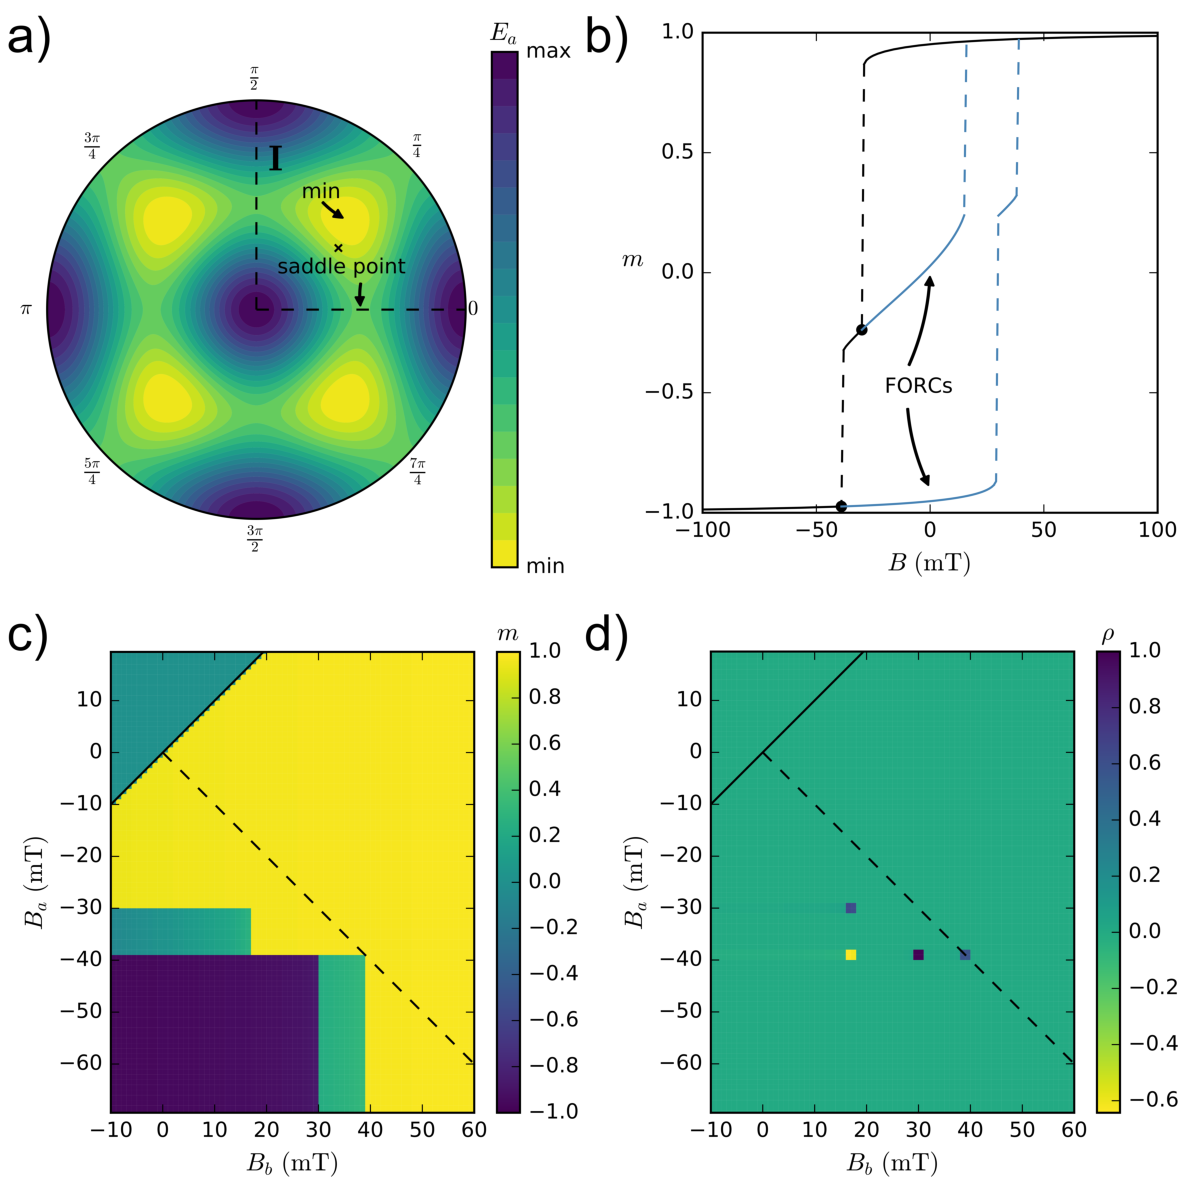
\includegraphics[width=\textwidth]{research-2/figs/FIG01.pdf}
\caption[Basic FORC modelling concepts]{Basic concepts. a) Energy landscape projection in polar coordinates for $K_1<0,\, K_2=0$; b) a complete set of FORCs for $\theta ,\,\phi$ as marked by the $\boldsymbol{\times}$ in a); c) the reduced magnetisation $m(B_b=\mu_0 H_b, B_a=\mu_0 H_a)$; d) the corresponding FORC distribution (normalised) with SF=1. The FORC distribution fronts and tails coincide with the sharp edges of $m(B_b, B_a)$.}
\label{FIG01}
\end{figure}
\par
A SF=1 was used to calculate the FORC distribution of each individual particle to limit the smoothing and retain the delta-like profile of the FORC distribution as much as possible (Figure \ref{FIG01}(d).) In this manner, FORC distributions were obtained by adding those of each individual particle instead of calculating $\rho$ on the ensemble magnetic response; essentially, this is what allows to remove the irreversible contribution from the FORC distribution of each particle and obtain the purely reversible FORC signal. FORC diagrams with SF=4 were also calculated; in these the reversible and irreversible contributions are mixed. Using a nonlinear scale, however, it is possible to discern the low-valued reversible contributions.\par

\subsection{Backtracking line-search gradient-descent method}\label{grad method}
A small spherical ferromagnetic particle in the single-domain (SD) state is modelled as a magnetic dipole with constant magnitude $|\boldsymbol{M}| = M_s$, the saturation magnetisation of the material. The magnetic Gibbs free-energy density of the particle is then the sum of the magnetocrystalline anisotropy (MCA) and the external field energy densities:
\begin{equation}\label{EQ:ENERGY}
E = E_a +E_z
\end{equation}
with
\begin{align}
E_a &= \frac{K_1}{2}\sum_{i\neq j}\alpha_i^2 \alpha_j^2 + K_2 \prod_i \alpha_i^2,\\
E_z &= - M_s\left( \boldsymbol{m} \cdot \boldsymbol{B}\right) = -M_sB \left( \alpha\chi + \beta\psi + \gamma\omega\right);
\end{align}
where $\alpha_i = \left(\alpha,\,\beta,\,\gamma\right)$ are the direction cosines of the reduced magnetisation $\boldsymbol{m} = \boldsymbol{M}/|\boldsymbol{M}|$ and $\left(\chi,\,\psi,\,\omega\right)$ those of the external field $\boldsymbol{B}=\mu_0 \boldsymbol{H}$; $K_1$ and $K_2$ the first and second MCA constants. From thermodynamics it is known that a system is spontaneously driven towards states with locally minimal Gibbs free-energy. Therefore, we are concerned with finding the LEM of the function $E=E(\boldsymbol{m},\,\boldsymbol{B})$.\par

Since the reduced magnetisation vector is unitary, it is natural to express the energy in the spherical coordinate system $E=E(\boldsymbol{m}=\boldsymbol{m}(\theta,\,\phi),\, \boldsymbol{B})$ ($\theta, \phi$ the polar and azimuthal angles, respectively):
\begin{align}
E_a &= K_1 \sin^2\theta\left[ \cos^2\theta + \left( \sin\theta\cos\phi\sin\phi\right)^2 \right] \nonumber \\
    &+ K_2\sin^2\theta \left( \sin\theta\cos\theta\sin\phi\cos\phi \right)^2, \label{EQ:ENERGY anis} \\
E_z &= -M_sB \left( \chi\sin\theta\cos\phi + \psi\sin\theta\sin\phi + \omega\cos\theta\right). \label{EQ:ENERGY ext}
\end{align}
$E_a$ minima and maxima lie along crystallographic orientations depending on the sign of $K_1,\,\,K_2$ and the ratio $|K_2| / |K_1|$. For $K_1<0$ ($K_2=0$) the easy axes (minima) are the $<$111$>$ and the hard (maxima) the $<$100$>$; the $<$110$>$ are saddle points (Fig. \ref{FIG01}(a)). When $K_1>0$ ($K_2=0$) instead, the easy axes become the $<$100$>$ and the hard the $<$111$>$ while the $<$110$>$ remain as saddle points.\par

From eq. (\ref{EQ:ENERGY}), (\ref{EQ:ENERGY anis}--\ref{EQ:ENERGY ext}), the gradient is then
\begin{align}
  \nabla E &= \hat{e}_\theta \left( E_a + E_z \right)_\theta + \hat{e}_\phi \left( E_a + E_z \right)_\phi  \nonumber \\
           &= \hat{e}_\theta \left( (E_a)_\theta + (E_z)_\theta \right) + \hat{e}_\phi \left( (E_a)_\phi + (E_z)_\phi \right);
\end{align}
where
\begin{align}
( E_a )_\theta &= 2\sin\theta\cos\theta\left\{ K_1  \left[ 2\left( \sin\theta\sin\phi\cos\phi \right)^2 \right. \right. \nonumber \\
             &- \left. \sin^2 \theta + \cos^2 \theta \right] \nonumber \\
             &+ \left. K_2 \left[ 2( \sin\theta\cos\theta\sin\phi\cos\phi )^2 - \sin^4\theta \right] \right\}, \\
( E_z )_\theta &= - M_s B ( \chi\cos\theta\cos\phi + \psi\cos\theta\sin\phi - \omega\sin\theta ) \\
( E_a )_\phi &= 2\sin^4\theta\sin\phi\cos\phi \left( K_1+K_2\cos^2\theta\right) \nonumber \\
            &\times \left( - \sin^2\phi + \cos^2\phi \right) \\
( E_z )_\phi &= -M_s B\sin\theta \left( - \chi\sin\phi + \psi\cos\phi \right).
\end{align}
\par
A backtracking line-search gradient-descent method \citep{Armijo1966} was implemented to simulate hysteresis loops and first-order reversal curves of nanomagnets with cubic MCA. The Armijo-Goldstein control parameters $c=1\times10^-4$, $\tau=1/2$ were used in this study. These ensure that the minimiser follows the gradient-descent direction very closely (Fig. \ref{FIG02}).
\begin{figure}
\includegraphics[width=\textwidth]{research-2/figs/FIG02.pdf}
\caption[The behaviour of the minimiser during irreversible motion]{The behaviour of the minimiser during irreversible motion along the main branch of the FORCs shown in Fig. \ref{FIG01}(b). a) When the field is -30$\,$mT the magnetisation irreversibly rotates from its position in the positive octant ($x,y,z>0$) (grey dot) to the one with $z<0$, where a local energy minimum is found (black dot). As the field strength is further increased the local energy minimum becomes more shallow until b) at -39$\,$mT an energy gradient causes the irreversible motion to the negative octant ($x,y,z<0$) where saturation occurs.}
\label{FIG02}
\end{figure}
\par

\section{Results and Discussion}
The calculated FORCs for a given field orientation are shown in Fig. \ref{FIG01}(b). Fig. \ref{FIG01}(c--d) shows the magnetisation as a function of $(B_b, B_a)$ and the corresponding FORC diagram (normalised). It is seen that the distribution is a collection of tail/front pairs like Eqn. \ref{forc hysteron} along the discontinuities in $m(B_b, B_a)$. A negative delta-like source at $(B_b=17\,\mathrm{mT},\,B_a=-39\,\mathrm{mT})$ is caused by the curve with $B_a=-38\,$mT going back to positive saturation at $B_b=17\,$mT while the one with $B_a=-39\,$mT remains in its negative saturation state up to $B_b=30\,$mT. These type of strong, highly-localised FORC distribution negative sources are then due to irreversible events on different FORCs. These strong, negative delta-like sources cannot occur in uniaxial particles which have only one irreversible event along the hysteresis main branch; low-valued negative delta-like sources are possible in uniaxial systems for the particles with easy axis almost normal to the applied field which experience very small irreversible upward jumps \citep{Stoner1948,Newell2005}.\par

The particles that have an easy axis alignment closer to the external field produce highly-symmetric, hysteron-like hysteresis curves which are responsible for the accumulation of positive delta-like sources along the central ridge (the line $H_a=-H_b$). The material with the highest coercivities $B_\text{C}$ was found to be greigite, with $B_\text{C}$ as high as 80$\,$mT for particles with an easy axis closely aligned with the applied field. Iron has coercivities as high as 50$\,$mT. The lowest coercivities for iron and greigite are 16$\,$mT.\par

The FORC distributions (Fig. \ref{FIG03}) show similar patterns for both materials. Greigite (Figs. \ref{FIG03}(a--b)), with its high coercivity, accumulates positive delta-like sources along the central ridge from 26$\,$mT up to 80$\,$mT. A region $\{(B_b,\,B_a):\,15\,\text{mT}< B_b < 18\,\text{mT},\, -26\,\text{mT}< B_a < -16\,\text{mT}\}$ with the highest $\rho^{*}=\rho/\max (\rho)$ values is caused by a cascade of particles with easy axis far from the field orientation switching at low $B_a$ values to intermediate states and back to positive saturation at $B_b < |B_a|$. These irreversible events then cause the accumulation of negative delta-like sources along a negative-valued vertical ridge. To the right of this, another (smaller) negative feature is produced by the irreversible events of particles undergoing hysteresis loops with more than two jumps, which corresponds to the fraction of particles with hard axes very closely aligned with the external field. Comparing Figs. \ref{FIG03}(a--b) it is clear that the negative ridge in the FORC distribution disappears in the purely reversible map and is therefore caused only by irreversible events.
\begin{figure}
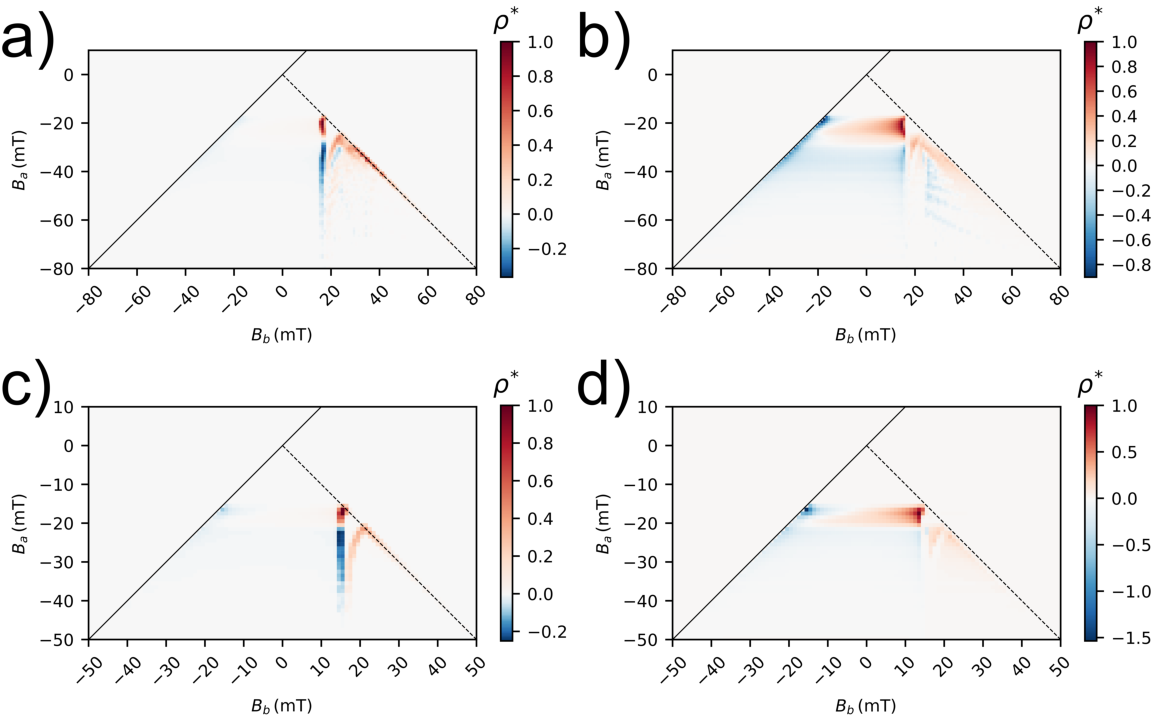
\includegraphics[width=\textwidth]{research-2/figs/FIG03.pdf}
\caption[FORC distribution heat maps (dipolar model)]{FORC distribution heat maps (normalised). a) Greigite and b) its purely reversible part; same for c,d) iron. Note the different scales for each material. Greigite ($K_1 < 0$) and iron ($K_1>0$) show very similar patterns. However, iron distintictively shows no negative sources, either reversible or irreversible, to the right of the negative-valued vertical ridge.}
\label{FIG03}
\end{figure}
\par
For iron (Figs. \ref{FIG03}(c--d)), the pattern formation is similar, if only with the position and width of the features changing. However, a fundamental difference is that for $K_1>0$ there is not an appreciable fraction of particles with hysteresis loops with more than two irreversible events. This is manifested in the FORC distribution by the absence of negative sources to the right of the negative vertical ridge.\par

FORC diagrams are usually presented as contour plots of the FORC distribution with higher values of the smoothing factor. The usual plotting axes are the transformed $B_c = (B_b - B_a)/2$, $B_u = (B_b + B_a)/2$; in this manner, FORC diagrams were calculated (Fig. \ref{FIG04}). The patterns show very similar pattern formation. The higher SF has the effect not only of smoothing the distribution but can also make the reversible information more apparent, especially if nonlinear scales are used for the contours of lower values.
\begin{figure}
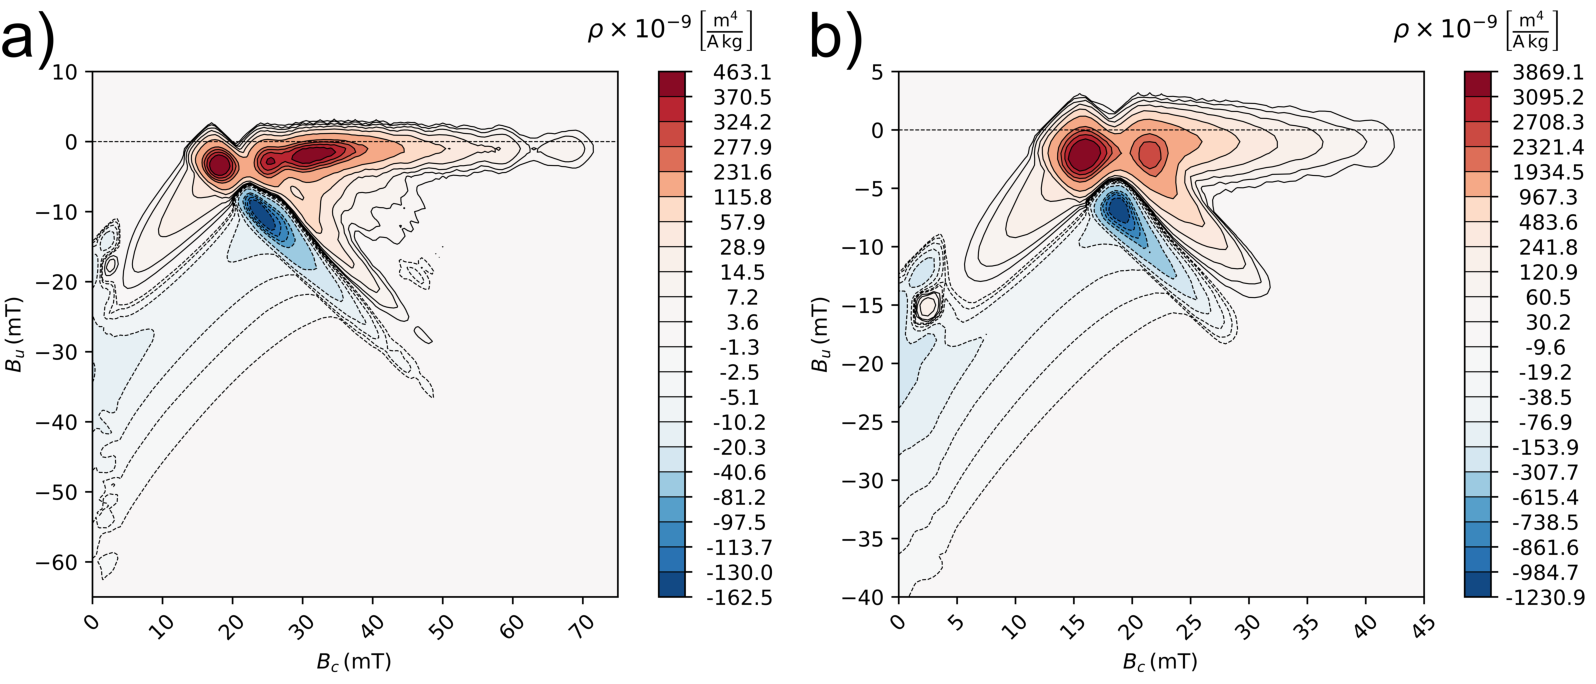
\includegraphics[width=\textwidth]{research-2/figs/FIG04.pdf}
\caption[FORC diagrams (dipolar model)]{The FORC diagrams. a) Greigite (SF=4); b) iron (SF=4). Note the different scales. The pattern formations are very similar in overall shape. Contour lines are plotted using a combination of linear and nonlinear scales at $(2^{-7},\ldots, 2^{-1},0.6, 0.7, 0.8)\times (\max (\rho), \min (\rho))$.}
\label{FIG04}
\end{figure}
\par
The position of the features in the FORC diagrams is slightly offset from being centered around the $B_u=0$ axis. This has been observed before in both measured and modelled FORC diagrams. \citet{Newell2005} attributes this to either a numerical artifact introduced by the least-square fitting-type calculation of the FORC distribution or to thermal effects. However, at least in this study, this should be attributed to the reversible contributions accumulating just below the central ridge.\par

The FORC diagrams obtained here for noninteracting ensembles of SD particles with cubic MCA shows good agreement with the weakly interacting ensembles of \citet{Harrison2014} as far as overall shape, e.g., the tilted negative ridge (Fig. \ref{FIG04}). The elongated, negative-valued ridge is highly significative and related to the presence of intermediate states, i.e., more than one irreversible event along the hysteresis curve. Uniaxial particles cannot produce this type of FORC distribution sources, so this is possibly a unique magnetic fingerprint of noninteracting to weakly interacting, coherent-rotating SD particles with cubic MCA. The tilted negative ridge has been observed before in FORC measurements of synthetic and natural greigite samples \citep{Roberts2011} and meteoritic samples \citep{Acton2007}.\par

FORC diagrams are usually presented normalised and their interpretation is usually qualitative. We find that iron produces much stronger FORC distribution sources per mass unit than greigite (Fig. \ref{FIG04}). It is possible that the strength of the negative ridge can be used in the future for quantitative studies, but more work is needed in this direction.\par

\section{Conclusion}
The FORC distribution and diagram of noninteracting dispersions of SD particles with cubic MCA was calculated. The numerical algorithm was found to be robust and fast. It is important that the minimiser takes sensible steps in order to closely follow the gradient-descent direction and not end up in local energy minima across energy barriers; the Armijo-Goldstein control parameters used in this study ensure these conditions.\par

The mechanism behind the pattern formation on the FORC diagram of dilute dispersions of SD particles with cubic MCA was identified. The FORC signals due to the reversible and irreversible motions were determined. The FORC diagram pattern of noninteracting to weakly interacting, cubic MCA SD particle ensembles are robust, which supports the idea of FORC diagram use for the identification of a noninteracting to weakly-interacting fraction of SD particles with cubic MCA.\par

The elongated negative ridge can possibly be interpreted as the FORC signal unique to noninteracting to weakly-interacting SD cubic MCA particles. Identification of this signal should be straightforward since its noninteracting nature means that it is essentially additive. Experimental work with dilute dispersions of fine particles of greigite, iron, magnetite or other magnetic minerals with a cubic MCA can provide answers to some of these open questions.\par

%%%% REFERENCES
\renewcommand\bibname{{References}}
\bibliographystyle{elsarticle-harv}
\bibliography{references}

